\documentclass[11pt]{article}
\usepackage{amsmath}
\usepackage{graphicx}

\newcommand{\infinity}{\infty}



\title{Notes for Math Equation}
\author{Synferlo}
\date{August 28, 2020}


\begin{document}
\maketitle

    \newpage
    
    \section{Basic Math Structure}
        \subsection{Inline math}
            Given production function $f(L,K)=L^\alpha K^\beta$,
            which is a function of input labor and capital.


        \subsection{Newline math}
            Given production function $$f(L,K)=L^\alpha K^\beta,$$
            which is a function of input labor and capital.


        \subsection{Equation Environment}
            Given production function
            %这里\begin{equation*}中的*表示我不想用序号标记这个公式
            \begin{equation*}
                f(L,K)=L^\alpha K^\beta,
            \end{equation*}
            which is a function of input labor and capital.


        \subsection{Alignment}
            %使用align环境每一行公式后必须使用\\换行符进行间隔。
            Consider the Euler equation and capital accumulation as the following:
            \begin{align}
                U(C_{t})&=\beta\times U(C_{t+1})\times[1+f(k_{t})-\delta]\\
                K_{t+1}&=(1-\delta)K_{t} + I_{t}
            \end{align}\\



    
    \section{Basic Math Notation}
        \subsection{Fraction}
        %输入分式时,使用 \frac{分子}{分母} 格式
        %分式嵌套时,可以用 \cfrac{分子}{分母}确保字体不会变换
        Define function $f(x)$ as following:
        $$ f(x) = \frac{1}{x} $$
        $$ \varepsilon_{ii} = \cfrac{\cfrac{\partial X_i}{X_i}} {\cfrac{\partial P_i}{P_i}} $$

        %如果分式的分子分母只有一个字符,则不需要加{}
        $$ f(x) = \frac12$$
        $$ f(x) = \frac1x$$


        \subsection{Square Root}
        %使用 \sqrt 时,如果后面是复杂的多项式,则用{}将内容括起来
        $$ x = \sqrt3 $$
        $$ x = \sqrt[2]{3} $$
        $$ x = \frac{1}{\sqrt{3}} $$
        $$ x = \sqrt{a+b+y^2} $$


        \subsection{Power and Integral}
        Define a quadratic function $f(x)$ as following:
        $$ f(x) = x^2 $$

        %书写积分时候,使用 \int表示integral,后面接上限,而后使用 _ 连接下限
        Given the expectation $E(x)$,
        $$ E(X) = \int^\infinity_{-\infinity} X f_{x}(x)dx$$

        Given interval $[a, b]$, 
        $$ E(X) = \iiint ^a _b X f_x(x)dx $$

        \subsection{Summation}
        % 书写加总符号的时候,使用 \sum 表示加总符号,而使用 _{下限} 跟下限, ^{} 跟上限
        % 个人规范,以后任何形式上下标,均从下标开始写起,上、下标、后续公式之间以空格隔开!!
        For discrete RVs, the expectation is defined as,
        $$ E(X) = n ^{-1} \times \sum_{i = 1} ^N {X_i}. $$
        Or
        $$ E(X) = \frac{1}{n} \times \sum _{i = 1} ^N {X_i}. $$

        %另外,也可以通过添加 \nolimits 或 \limits 改变形态
        $$ E(X) = n^{-1} \times \sum\nolimits_{i = 1} ^N {X_i}. $$

        %当你觉得空间不够的时候可以使用四个$当空行使用啊哈哈哈
        $$$$
        %当限制条件很多,一行写不下的时候可以使用一下方法
        The utility maximization problem becomes
        $$ \max_{c_s,k_s \atop l_s} \sum_{s = 0} ^\infinity {\beta^{s-t} U(C_s)}$$

        Or you can use this way:
        $$ \max_{\substack{c_s, k_s\\l_s}} \sum_{s = 0} ^\infinity {\beta^{s-t}U(C_s)} $$

        
        \subsection{Production}
        %连乘使用 \prod 命令, 使用 _ 表示下标,^ 表示上标
        The generalized form for Cobb-Douglas utility function is
        $$ U(X_1,...,X_n) = \prod_{i = 1} ^n X_i^{\alpha_i} $$

        For dot production(matrix)
        $$ X_1 \cdot Y_1$$


        \subsection{Limitation}         
        %使用 \lim 命令完成求极限输出。 \lim_{n \to x} 表示当n趋近于x时。注意一定要是 \to !!
        The Variance of $E(x)$ is defined by
        \begin{align*}
            Var(E(X)) &= Var (n^{-1} \times \sum_{i = 1} ^N {X_i})\\
            & = \frac{1}{n^2} \times \sum_{i = 1} ^N {Var({X_i})}\\
            & = \frac{\sigma^2}{n}
        \end{align*}
        When n goes to infinity,
        \begin{align*}
            \lim_{n \to \infinity} Var(E(X)) & = \lim_{n \to \infinity} \frac{\sigma^2}{n}\\
            & = 0
        \end{align*}

        
        \subsection{Differentiation}
        % 偏导符号命令: \partial
        % 上三角符号:   \Delta
        The own price elasticity for good i is defined by
        $$ \epsilon_{ii} = \frac{\partial X_i}{\partial P_i} \frac{P_i}{X_i}$$
        \begin{align*}
            \epsilon_{ii} &= \frac{\partial X_i}{\partial P_i} \frac{P_i}{X_i}\\
            & = \cfrac{\cfrac{\partial X_i}{X_i}} {\cfrac{\partial P_i}{P_i}}\\
            & = \frac{lnX_i}{lnP_i}\\
            & = \frac{\Delta X_i}{\Delta P_i}
        \end{align*}
        

        \subsection{Binomial Operation}
         Binomial distribution with density function
         $$ f(x;\theta) = \binom{n}{x} \theta^x (1-\theta)^{n-x} $$
         where $\binom{n}{x} = \frac{n!}{(n-x)!x!} $
         $$$$
         Or you can right in this method,
         $${n \choose x}$$


        \subsection{Convergence}
        Denote $\mu_r'$ converge to standard normal distribution in distribution as the following:
        $$\mu_r' \xrightarrow{d} N(0, 1)$$
        
        \subsection{Head-Notation}
        \begin{equation*}
            y = x\hat{\beta} + \varepsilon
        \end{equation*}

        Average of x is $\bar{x}$
        

        \subsection{Density Function}
        $$
        f(x;\theta) = 
        \begin{cases}
            \frac{1}{b-a} \quad &if x\in[a,b]\\
            \emptyset \quad &O.W
        \end{cases}
        $$


        \subsection{Matrix}

        $$\begin{bmatrix}
            1 & 2 & 1 \\
            3 & 8 & 1 \\
            5 & 1 & 1

        \end{bmatrix}$$
        $$$$
        $$\begin{pmatrix}
            1 & 2 & 1 \\
            3 & 8 & 1 \\
            5 & 1 & 1
        \end{pmatrix}$$

        $$
        \begin{pmatrix}
            1 & x_{11} & x_{12} \cdots x_{1k}\\
            1 & x_{21} & x_{22} \cdots x_{2k}\\
            \vdots & \vdots & \ddots \vdots\\
            1 & x_{n1} & x_{n2} \cdots x_{nk}\\
            
        \end{pmatrix}
        $$
        $$$$

        $$
        A = 
        \begin{pmatrix}
            \begin{matrix}
                1 & 0\\
                0 & 1
            \end{matrix}
            & 0 \\
            0 & 
            \begin{matrix}
                1 & 0\\
                0 & 1
            \end{matrix}
        \end{pmatrix}
        $$


        $$
        B = 
        \begin{pmatrix}
            \begin{matrix}
                1 & 0\\
                0 & 1
            \end{matrix}
            & 0\\
            0 &
            \begin{matrix}
                1 & 0\\
                0 & 1
            \end{matrix}
        \end{pmatrix}
        $$


        \subsection{Bracket}
        %公式复杂的时候,比如有多个分式嵌套时,使用 \left( 和 \right) 来时括号自动调整大小

        $$
        \lim_{x \to 0} \left(\frac{a^x + b^x + c^x}{3} \right)^\frac1x
        $$

        This is a \textbf{fantastic} way to formalized the bracket in your equation.

    \section{Insert Materials}

        \subsection{Graphics}
        % 使用scale来调整缩放百分比
        % 使用\centering来规定居中对齐图片
        \centering
        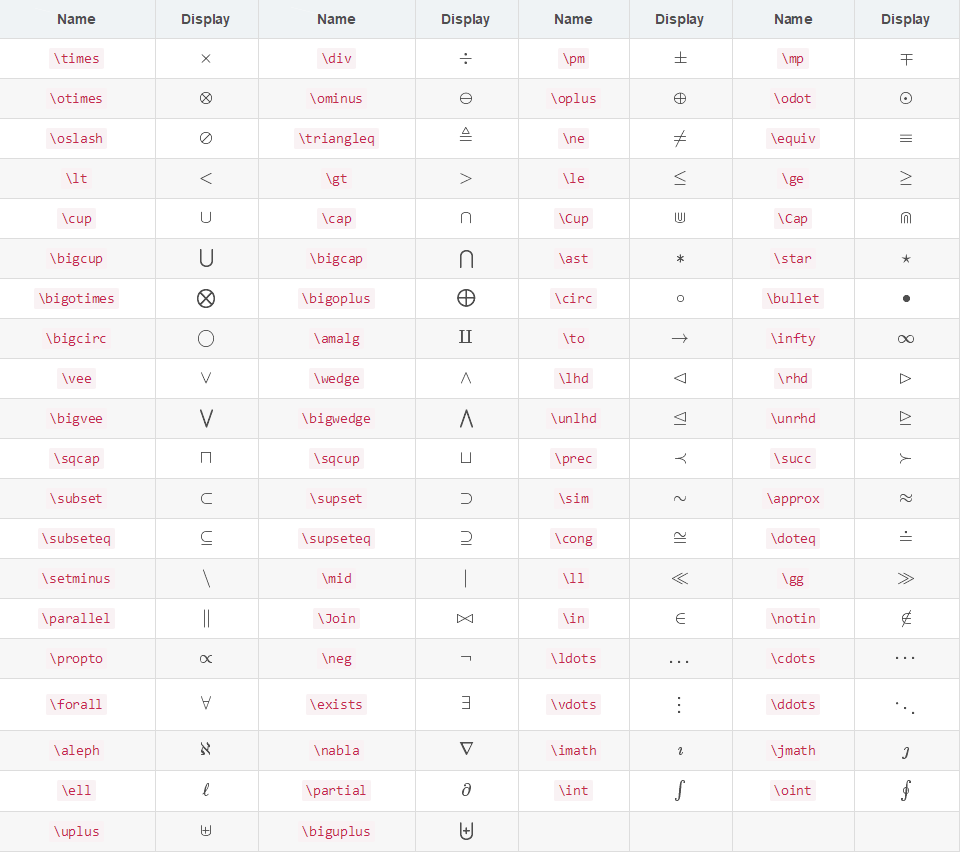
\includegraphics[scale = 0.2]{Operation_Sign.png}






\end{document}
